
\begin{figure}[h]
    \centering
    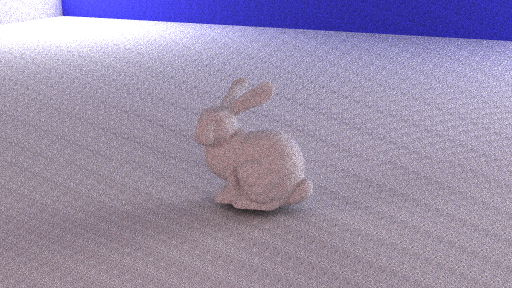
\includegraphics[width=0.8\columnwidth]{render_stanford_bunny_dummy.png}
    \caption{Stanford bunny rendered with a simple path tracer algorithm.}
    \label{fig:stanford_bunny_dummy}
\end{figure}

\begin{figure}[h]
    \centering
    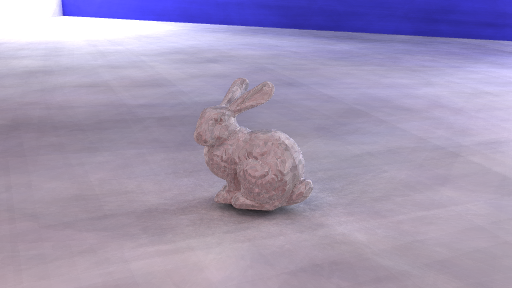
\includegraphics[width=0.8\columnwidth]{render_stanford_bunny_cpt.png}
    \caption{Stanford bunny rendered with a coherent path tracer algorithm.}
    \label{fig:stanford_bunny_cpt}
\end{figure}

\begin{figure}[H]
    \tiny
    \centering
    \begin{tabular}{ | l | c | c | }

        \hline
        Algorithm used & Bunny \\
        \hline
        Simple path tracer & 224.0ns \\
        Coherent path tracer & 101.9ns \\
        \hline

    \end{tabular}
    \caption{
        Per ray rendering time comparaison between a simple path tracer
        algorithm and a coherent path tracer (resolution of 512~x~288; 512
        sample per pixels; 9 recursive raies per samples).
    }
    \label{table:cpt_compare}
\end{figure}
